\documentclass[12pt]{article}
\usepackage{graphicx,amssymb,amsmath,subfigure}

\oddsidemargin  -0.5 cm
\evensidemargin 0.0 cm
\textwidth      6.5in
\headheight     0.0in
\topmargin      -1 cm
\textheight=9in

\renewcommand{\arraystretch}{1.25}

\begin{document}

\section{Alignment Method}

It's too late at night for me to write a proper document, so I'm just
going to write enough here for you to understand what I'm doing.  It
will be the basis for a better write-up later.

The goal is to align as many degrees of freedom as possible using the
information provided by residuals between tracks and hits.  To get the
most information out of a track's intersection with a chamber, we
first combine all of its residuals into a super-residual which
expresses the difference in position between the track and all of its
hits and the difference in angle between the track and all of its
hits.  We compute this position difference and angle difference from
an analytic linear fit, e.g.\ for $\Delta x_i$ residuals on layers of
fixed $z_i$,
\begin{eqnarray}
\mbox{position difference } = \mbox{ }a &=& \frac{1}{\mbox{denominator}} \left(\sum\frac{z_i^2}{\sigma_i^2} \sum\frac{\Delta x_i}{\sigma_i^2} - \sum\frac{z_i}{\sigma_i^2} \sum\frac{z_i \Delta x_i}{\sigma_i^2}\right) \\
\mbox{angle difference } = \mbox{ }b &=& \frac{1}{\mbox{denominator}} \left(\sum\frac{1}{\sigma_i^2} \sum\frac{z_i \Delta x_i}{\sigma_i^2} - \sum\frac{z_i}{\sigma_i^2} \sum\frac{\Delta x_i}{\sigma_i^2}\right) \\
\mbox{where denominator} &=& \sum\frac{1}{\sigma_i^2}
\sum\frac{z_i^2}{\sigma_i^2} - \left(\sum\frac{z_i}{\sigma_i^2}\right)^2 \\
\mbox{with } \chi^2/N_{\mbox{\scriptsize dof}} &=& \frac{1}{N_{\mbox{\scriptsize hits}} - 2} \sum \frac{\Delta (x_i - a - z_i \, b)^2}{\sigma_i^2} \mbox{ as a quality parameter.}
\label{eqn:superresiduals}
\end{eqnarray}
Super-residuals are more precise than segment residuals because we
only assume that the difference between the muon's path and the
track's propagation is linear.  The muon may be following a curved
path, for example in ME1/1, where $|\vec{B}| > 2.5$~T.

{\it (Editorial comment: I think this method provides more information
  than using the 1-D hits individually, because it inserts the
  information that the hits in the same chamber have smaller relative
  errors than hits in different chambers.)}

DT chambers in stations 1, 2, and 3 are capable of measuring local $x$
and $y$ coordinates, while DT chambers in station 4 can measure only
local $x$.  CSC chambers can in principle measure $x$ and $y$ using
intersections of cathode strips and anode wires, but the wires are
ganged in 5~cm groups, which is too large of a granularity for
alignment.  (The chambers are already better aligned than that.)
Moreover, the stips are not parallel, but fan radially from the
beamline, so that they are directly sensitive to the curvilinear
coordinate $r\phi$ rather than the cartesian $x$
(Fig~\ref{fig:csc_localrphi}).  To use the chamber's best information,
we extract $r\phi$ residuals from the CSCs.  Combining these residuals
into super-residuals using the method of Eqn~\ref{eqn:superresiduals},
we obtain
\begin{itemize}
\item $\Delta x$ and $\Delta y$ position super-residuals and $\Delta
  \frac{dx}{dz}$ and $\Delta \frac{dy}{dz}$ angular super-residuals
  from chambers in barrel stations 1, 2, and 3,
\item $\Delta x$ position and $\Delta \frac{dx}{dz}$ angular
  super-residuals from chambers in barrel station 4, and
\item $\Delta r\phi$ position and $\Delta \frac{dr\phi}{dz}$ angular
  super-residuals from CSC chambers.
\end{itemize}

\begin{figure}
\begin{center} 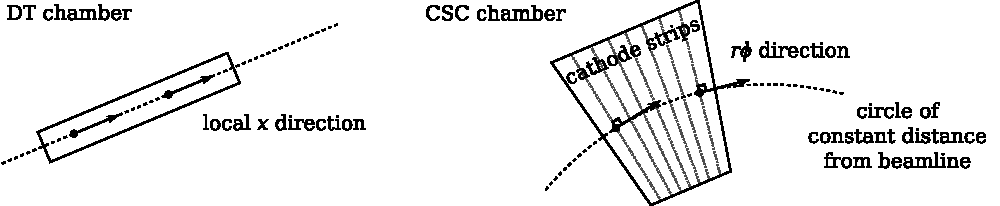
\includegraphics{strip_direction.pdf} \end{center}
\caption{Local $x$ and $y$ coordinates in DT chambers are rectilinear, but the fanning of CSC strips makes it more convenient to measure residuals and align CSCs in curvilinear $r\phi$. \label{fig:csc_localrphi}}
\end{figure}

It is easy to see that an offset in $\Delta x$ super-residuals is an
indication of a $\delta_x$ misalignment, and with some geometry
(Fig~\ref{fig:phiz_zpos}), relationships between the six alignment
parameters ($\delta_x$, $\delta_y$, $\delta_z$, $\delta_{\phi_x}$,
$\delta_{\phi_y}$, and $\delta_{\phi_z}$) and the super-residuals can
be derived.  The complete set of relationships can be written as a
matrix, expressing the geometric correction each alignment parameter
imposes upon the residuals.

\begin{equation}
\renewcommand{\arraystretch}{2.5}
\left(\begin{array}{c}
{\Delta x}^{\mbox{\scriptsize geom}} \\
{\Delta y}^{\mbox{\scriptsize geom}} \\
{\Delta \dfrac{dx}{dz}}^{\mbox{\scriptsize geom}} \\
{\Delta \dfrac{dy}{dz}}^{\mbox{\scriptsize geom}} \\
\end{array}\right)
=
{\renewcommand{\arraystretch}{2.5}
\left(\begin{array}{c c c c c c}
1 & 0 & -\dfrac{dx}{dz} & -y \dfrac{dx}{dz} & x \dfrac{dx}{dz} & -y \\
0 & 1 & -\dfrac{dy}{dz} & -y \dfrac{dy}{dz} & x \dfrac{dy}{dz} & x \\
0 & 0 & 0 & -\dfrac{dx}{dz} \dfrac{dy}{dz} & 1 + \left(\dfrac{dx}{dz}\right)^2 & -\dfrac{dy}{dz} \\
0 & 0 & 0 & -1 - \left(\dfrac{dy}{dz}\right)^2 & \dfrac{dx}{dz}\dfrac{dy}{dz} & \dfrac{dx}{dz}
\end{array}\right)}
\renewcommand{\arraystretch}{1.7}
\left(\begin{array}{c}
\delta_x \\
\delta_y \\
\delta_z \\
\delta_{\phi_x} \\
\delta_{\phi_y} \\
\delta_{\phi_z}
\end{array}\right)
\label{eqn:dtmatrix}
\end{equation}
where $x$, $y$, $\frac{dx}{dz}$, and $\frac{dy}{dz}$ denote the impact
point and entrance angle of the track.  The top two rows are the
``Karimaki derivatives'' used in the tracker to align all 6 degrees of
freedom with two position residuals.  The addition of super-residual
angles $\Delta \frac{dx}{dz}$ and $\Delta \frac{dy}{dz}$ adds
significance to $\delta_{\phi_y}$ and $\delta_{\phi_x}$ alignments,
respectively, and all four observables contribute roughly equally to
our determination of $\delta_{\phi_z}$.

\begin{figure}
\subfigure[Linear relationship between $\Delta x$ residuals, $\delta \phi_z$ misalignment, and $y$ track position: \mbox{${\Delta x}^{\mbox{\scriptsize geom}} = y \, \delta_{\phi_z}$}]{\begin{minipage}{0.4\linewidth} \begin{center} 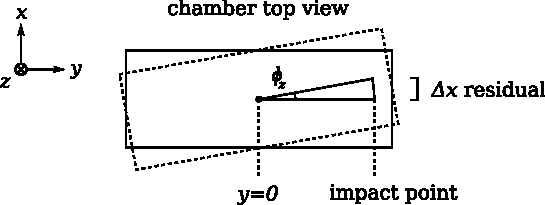
\includegraphics{phiz_diagram.pdf} \end{center} \vspace{0.2 cm} \end{minipage}} \hfill \subfigure[Linear relationship between $\Delta x$ residuals, $\delta z$ misalignment, and $dx/dz$ track angle: \mbox{${\Delta x}^{\mbox{\scriptsize geom}} = (dx/dz) \, \delta z$}]{\begin{minipage}{0.4\linewidth} \begin{center} 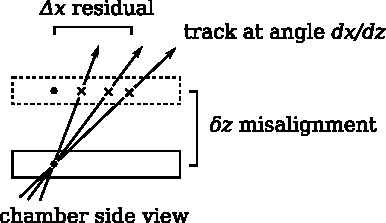
\includegraphics{zpos_diagram.pdf} \end{center} \vspace{0.2 cm} \end{minipage}}
\caption{Geometric arguments justifying two of the matrix elements in Eqn~\ref{eqn:dtmatrix} \label{fig:phiz_zpos}}
\end{figure}

In DT station 4, the lack of $\Delta y$ and $\Delta \frac{dy}{dz}$
residuals reduces the relationship to a submatrix of the above, and
$\delta_y$ cannot be aligned.
\begin{equation}
\renewcommand{\arraystretch}{3}
\left(\begin{array}{c}
{\Delta x}^{\mbox{\scriptsize geom}} \\
{\Delta \dfrac{dx}{dz}}^{\mbox{\scriptsize geom}} \\
\end{array}\right)
=
{\renewcommand{\arraystretch}{3}
\left(\begin{array}{c c c c c c}
1 & 0 & -\dfrac{dx}{dz} & -y \dfrac{dx}{dz} & x \dfrac{dx}{dz} & -y \\
0 & 0 & 0 & -\dfrac{dx}{dz} \dfrac{dy}{dz} & 1 + \left(\dfrac{dx}{dz}\right)^2 & -\dfrac{dy}{dz}
\end{array}\right)}
\renewcommand{\arraystretch}{1}
\left(\begin{array}{c}
\delta_x \\
\delta_y \\
\delta_z \\
\delta_{\phi_x} \\
\delta_{\phi_y} \\
\delta_{\phi_z}
\end{array}\right)
\label{eqn:dt4matrix}
\end{equation}

Though we treat CSCs as one-dimensional devices, the curvilinear
coordinate modifies its matrix from the above.  In principle, all 6
degrees of freedom are accessible to CSCs because strips near the
edges of the trapezoidal chambers measure linearly independent
combinations of $\delta_x$ and $\delta_y$.  Here is the CSC matrix
(keeping only important terms):
\begin{equation}
\renewcommand{\arraystretch}{3}
\left(\begin{array}{c}
{\Delta r\phi}^{\mbox{\scriptsize geom}} \\
{\Delta \dfrac{dr\phi}{dz}}^{\mbox{\scriptsize geom}} \\
\end{array}\right)
=
{\renewcommand{\arraystretch}{3}
\left(\begin{array}{c c c c c c}
1 & \left[ -\dfrac{x}{R} + 3\left(\dfrac{x}{R}\right)^3 \right] & -\dfrac{dx}{dz}  & -y \dfrac{dx}{dz} & x \dfrac{dx}{dz} & -y \\
0 & -\dfrac{dx}{dz}/(2R) & 0 & \left[ \dfrac{x}{R} - \dfrac{dx}{dz}\dfrac{dy}{dz} \right] & 1 + \left(\dfrac{dx}{dz}\right)^2 & -\dfrac{dy}{dz}
\end{array}\right)}
\renewcommand{\arraystretch}{1}
\left(\begin{array}{c}
\delta_x \\
\delta_y \\
\delta_z \\
\delta_{\phi_x} \\
\delta_{\phi_y} \\
\delta_{\phi_z}
\end{array}\right)
\label{eqn:cscmatrix}
\end{equation}
where $R$ is the distance to the convergence point of the strips,
nominally the beamline {\it (and assumed to be the beamline in the
  current version of the code)}.

Without measurement error, alignment would be a matter of solving
Eqns~\ref{eqn:dtmatrix}--\ref{eqn:cscmatrix} by matrix inversion.
Five effects broaden the residuals distributions:
\begin{itemize}
\item statistical propagation error from the tracker: the track
  coordinates are not perfectly known, and errors in direction and
  curvature grow linearly and quadratically with arclength along the
  track, respectively,
\item systematic misalignment error from the tracker, which might have
  a global pattern,
\item multiple-scattering in material, which adds Gaussian statistical
  error independently to each track,
\item single-scattering in material, which adds statistical error with
  a power-law distribution,
\item and chamber detector resolution, which is statistical and
  smaller than the above.
\end{itemize}
All of the statistical errors (everything except tracker misalignment)
can be expressed as a fit function.  The fact that single scattering
has a non-Gaussian distribution complicates the function somewhat, in
that the distribution must be a convolution of a Gaussian with a bell
curve with power-law tails: we choose a Lorentz-Cauchy distribution
for convenience.  The most important feature of the non-Gaussian part
of the fit is its reduced sensitivity to outlying events.

There is also a strong correlation between position residuals and
their corresponding angle residuals.  Tracks reconstructed with the
wrong direction for any reason (scattering, measurement error in the
tracker) will tend to be offset in position when they reach the
chamber by an amount proportional to the length of the track (see
Fig~\ref{fig:sawtooth_diagram}).  We can accommodate for this
correlation by adding fit parameters $\alpha_x$ and $\alpha_y$, for which
\begin{eqnarray}
{\Delta x}^{\mbox{\scriptsize average}} = \alpha_x \, {\Delta \frac{dx}{dz}}^{\mbox{\scriptsize average}} \\
{\Delta y}^{\mbox{\scriptsize average}} = \alpha_y \, {\Delta \frac{dy}{dz}}^{\mbox{\scriptsize average}}
\end{eqnarray}

\begin{figure}
\begin{center} 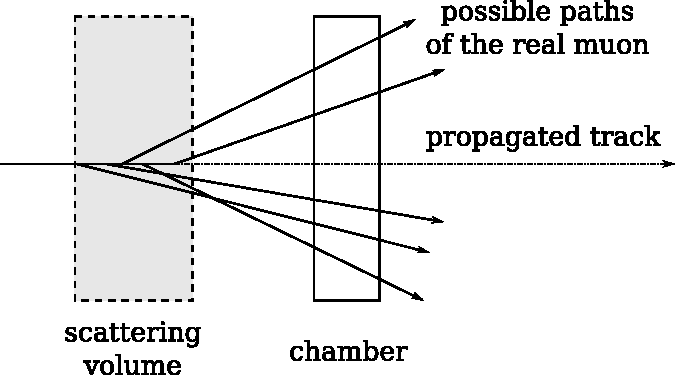
\includegraphics[height=4.5 cm]{sawtooth_diagram.pdf} \end{center}
\caption{Correlation between super-residual position error and angle error. \label{fig:sawtooth_diagram}}
\end{figure}

The fit function for a two-residual chamber such as DT station 4 and
the CSCs is
\begin{multline}
f_x(\Delta x; {\Delta x}^{\mbox{\scriptsize geom}}, \alpha_x, \Delta \frac{dx}{dz}, \sigma_x, \gamma_x) = \\
\int_{-\infty}^\infty
\frac{\gamma_x}{\pi}\left(\left(\Delta x - \xi - {\Delta x}^{\mbox{\scriptsize geom}} - \alpha_x \, \Delta \frac{dx}{dz}\right)^2 + {\gamma_x}^2\right)^{-1} \times 
\frac{1}{\sqrt{2\pi} \sigma_x} \exp\left(\frac{-\xi^2}{2 {\sigma_x}^2}\right) \, d\xi
\label{eqn:fitfunction1}
\end{multline}
\begin{multline}
g_x(\Delta \frac{dx}{dz}; {\Delta \frac{dx}{dz}}^{\mbox{\scriptsize geom}}, \sigma_{\frac{dx}{dz}}, \gamma_{\frac{dx}{dz}}) = \\
 \int_{-\infty}^\infty
\frac{\gamma_{\frac{dx}{dz}}}{\pi} \left(\left(\Delta \frac{dx}{dz} - \xi - {\Delta \frac{dx}{dz}}^{\mbox{\scriptsize geom}}\right)^2 + {\gamma_{\frac{dx}{dz}}}^2\right)^{-1} \times 
\frac{1}{\sqrt{2\pi} \sigma_{\frac{dx}{dz}}} \exp\left(\frac{-\xi^2}{2 {\sigma_{\frac{dx}{dz}}}^2}\right) \, d\xi
\label{eqn:fitfunction2}
\end{multline}
where we fit simultaneously for $f_x$ and $g_x$, implicitly including
all of the alignment parameters in ${\Delta x}^{\mbox{\scriptsize
    geom}}$ and ${\Delta \frac{dx}{dz}}^{\mbox{\scriptsize geom}}$.
DT chambers in stations 1, 2, and 3 are simultaneous fits for $f_x$,
$f_y$, $g_x$, and $g_y$, where $f_y$ and $g_y$ are defined similarly
to the above.  The width parameters $\sigma_x$,
$\sigma_{\frac{dx}{dz}}$, $\gamma_x$, and $\gamma_{\frac{dx}{dz}}$ are
the Gaussian width and the Lorentzian half-width at half maximum
(before convolution).  We use MINUIT to fit the observed
super-residuals to the above function in an unbinned maximum
likelihood fit, weighted by the inverse of super-residual quality
$(\chi^2/N_{\mbox{\scriptsize dof}})^{-1}$.

\section{Progress}

It was very important to include all alignment parameters for each
chamber into a single fit.  Excluding the $\Delta \frac{dx}{dz} =
-\frac{dy}{dz} \, \delta_{\phi_z}$ matrix element caused the fits to
not converge in random initial conditions, and an apparent confusion
between $\phi_y$ and $\phi_z$ in more controlled initial conditions.
On Wednesday, I was thinking of cobbling together a procedure which
aligns parameters in a particular order to make this sensitivity
irrelevant.  By including it in the fit function, it now becomes a
part of the measurement.  I have verified that this works.

The tests of Eqns~\ref{eqn:dtmatrix}--\ref{eqn:cscmatrix} were
extensive.  I discovered them via a mathematical model I made in
Python (therefore I know exactly what went into the calculation),
verified them in full CMSSW with the propagator intersecting alignable
chamber surfaces (therefore I know that I got all of the sign
conventions right), but without measurement error, and I have verified
that $\phi_y$ and $\phi_z$ are properly decoupled in the full Monte
Carlo.  This method correctly derived the Karimaki part of the matrix
(top two rows--- a HIP algorithm without super-residual angles, like
the one used in the tracker).

Trying to solve the fit-failure problem (below), I have tweaked the
fit function to a very high degree.  Weighting the super-residuals by
$(\chi^2/N_{\mbox{\scriptsize dof}})^{-1}$ has cleaned up the shape
considerably.  Consistency of hits with a straight line is a geometric
property, unlike hit uncertainty which can sometimes be ad-hoc and
describe Monte Carlo much better than data, so these weights are
unlikly to cause problems in data.

Still trying to solve the fit-failures, I also improved the numerical
stability of the fit function.  Convolutions are computationally
expensive, so it must be tabulated, with points between the table
entries computed by interpolation.  Rather than tabulate $f((x -
x_0)/\sigma,\mbox{ }\gamma/\sigma)$, I tabulated $\log f((x -
x_0)/\sigma,\mbox{ }\gamma/\sigma)$, interpolate in the log space, and
pass this to MINUIT as the log likelihood.  I also made the binning
ten times smaller in $\gamma/\sigma$.  Outside of the table
($\gamma/\sigma > 5$ and $(x-x_0)/\sigma > 50$) is now represented by a
pure Lorentzian, as that is what the curve limits to at those
extremes.  The transition from the table to pure Lorentzian is
relatively smooth, and most distributions have $\gamma/\sigma \approx
0.1$.

\section{Problems}

Many of the fits fail in MINUIT.  This problem has become more
frequent now that more parameters have been added to the fit, and
MINUIT's most frequent error messages are ``Hessian not positive
definite,'' and ``Machine precision isn't good enough to verify
convergence'' (implying a very shallow or a very non-smooth minimum).
However, this is still an issue when many of the parameters are fixed
at reasonable values (verified by plotting).  Fits are always given
reasonable starting values, computed from carefully truncated means
and standard deviations, and even a linear pre-fit to seed the largest
correlation (between $\Delta y$ and $\Delta \frac{dy}{dz}$).  The
problem also seems to be independent of whether the parameters are
given reasonable limits or not.  By default, I don't assign limits.

An important clue comes from the fact that replacing the fit function
(Eqns~\ref{eqn:fitfunction1}-\ref{eqn:fitfunction2}) with pure
Gaussian distributions always fits successfully (after
$\log(\exp(-x^2))$ was replaced by $-x^2$).  Unfortunately, the
distributions are not well described by Gaussians, and this can
seriously deteriorate the alignment results.  (Gaussian widths are
$\sim$10-100~mm.  The only way to get a good measurement of the peak
position is to do a very precise fit of the distribution.)  That's why
I revisited the formulation of the fit function, to make sure that it
is smooth.

Successful fits are a little disappointing, too: the alignment results
differ from MC truth by 3--5 standard deviations.  The geometry
matricies (Eqns~\ref{eqn:dtmatrix}--\ref{eqn:cscmatrix}) are
definitely not at fault, because they perform perfectly in the absence
of measurement error.  I suspect that whatever is causing the fit
failures (now about 50\%) is deteriorating the quality of the
successful fits--- that's why I now consider this an important issue.

If there's a robust way to find the maximum likelihood of the full fit
function without MINUIT, I'm willing to try it.  Scanning probably
won't work: the search space has too many dimensions for this to be
feasible.

A less important issue is that strict proportionality between $\Delta
x$ and $\Delta \frac{dx}{dz}$ and between $\Delta y$ and $\Delta
\frac{dy}{dz}$ doesn't model the data well.  The central region
($|\Delta \frac{dx}{dz}| < 5$~mrad and $|\Delta \frac{dy}{dz}| <
30$~mrad, about 1 standard deviation in each) is linear, but outside
of the is uncorrelated, so the whole distribution has more of an
S-shape.  2-d distributions and ntuple exploration doesn't reveal why
this is so.  It doesn't seem to be related to the fit failures, but it
might be important because this is the largest correlation, larger
than any alignment correlation.

\end{document}
